
\chapter{Robotic Platform for Mobile Manipulation}

This chapter describes the hardware configuration for the robotic platform used for the project.
The platform is composed of a mobile robot base, a robotic arm manipulator, sensors, 
a soft gripper actuator, 3D-printed mounts, batteries, power management systems, and other electronic devices.
The chapter will also discuss the issues faced during the development of the mobile manipulation platform.

\section{Mobile Robot Platform}

The mobile robot is an \textit{AgileX Scout 2.0} robot, depicted in Figure \ref{fig:c3_img01}.
This robot is a skid-steering robot, suitable for outdoor and indoor environments. 
Designed for robotics research and development, the Scout 2.0 is an unmanned ground vehicle (UGV). 
This autonomous mobile robot offers a robust mechanical design along with capable mobility performance. 
Built to endure diverse conditions, Scout 2.0 features rugged materials and protective casings, ensuring longevity
and reliability during missions. Scout 2.0 offers aluminum T-slot rails for secure mounting of external sensors or kits. 
On these rails, a variety of sensors, computers, or other devices are mounted, allowing the creation of a mobile robotic platform
for a wide range of applications, all powered by the \textbf{onboard battery system}.

It supports CAN bus protocol for connections and provides open-source SDK and software resources for expanded capabilities.
Its maximum speed is $1.5 m/s$, and it can carry a payload of $50$ kg. 
The robot is powered by a $24V$ battery, which provides a range of $15$ km maximum. 
The robot is controlled by a ROS-based software system, which allows the control of the robot's speed using a ROS topic
and receiving odometry data from the robot's encoders.

%Add the image of the robot
\begin{figure}[t]
	\centering
	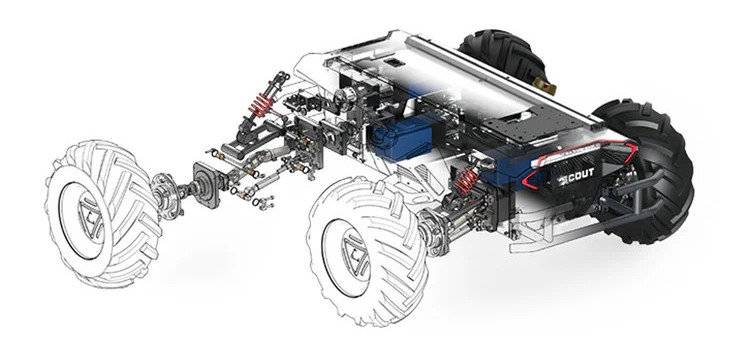
\includegraphics[width=1\textwidth]{chapter3_01.jpg}
	\captionsetup{width=1\linewidth}
	\caption{Scout 2.0 employs 200W brushless servo motors to drive each wheel independently. 
    Its double-wishbone suspension with shock absorbers ensures stability on rough terrain, 
    enabling it to tackle obstacles up to 10cm tall effortlessly.}
	\label{fig:c3_img01}
\end{figure}

On the mobile robot, an \textit{Intel NUC 12} computer \ref{fig:c3_img02} is mounted.
This \textbf{computer} is used to run all the control
software and the perception algorithms. The computer is connected to a switch, which is used to connect
the computer to the robotic arm's embedded control system, to the LiDAR sensor, and Wi-Fi hotspot router.
The mobile robot base is connected to the computer via the CAN bus, which is used to receive data from the robot's
encoders and send data to control the robot's speed and direction.
The on-board router is used to provide a Wi-Fi hotspot for remote access.
The computer's Wi-Fi is used to connect to the internet, allowing the robot to be controlled and monitored
remotely via a remote desktop connection. 
This computer has the following technical specifications:

\begin{itemize}
    \item Intel Core i7-12700H CPU
    \item 32GB DDR4 RAM
    \item 1TB NVMe SSD
    \item Intel Iris Xe Graphics
    \item Kubuntu 22.04 operating system
\end{itemize}

% Add the image of the computer
\begin{figure}[t]
    \centering
    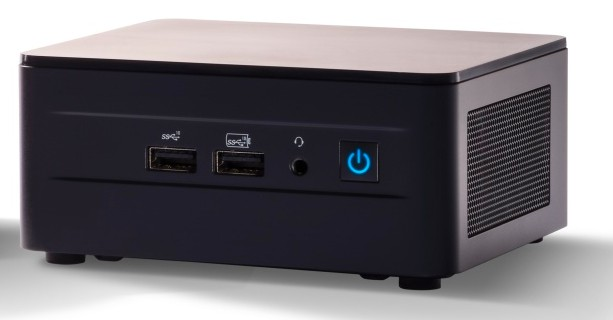
\includegraphics[width=0.6\textwidth]{chapter3_02.jpg}
    \captionsetup{width=1\linewidth}
    \caption{Intel NUC 12 computer mounted on the robot}
    \label{fig:c3_img02}
\end{figure}

The robot is equipped with an \textit{TP-Link Archer MR200} router and a \textit{Netgear GS108} switch.
The router was necessary to
establish a \textbf{remote connection} from a personal laptop to the robot's computer, allowing the control and monitoring
of the robot from a remote location. This is essential for the development of the project, as it allows to
work safely with the robot, ensuring that everything works smoothly and stopping the system in case of any
unexpected behavior or software crashes and malfunctions.

The robotic arm manipulator is also connected to the switch,
allowing the robot's computer to control the manipulator and receive data from its motors' encoders. 
The LiDAR is connected to the switch, allowing the robot's computer to receive pointcloud data from the LiDAR sensor,
at a fast transmission rate.
 
\section{Robotic Arm Manipulator}

The robotic arm manipulator used for the project is a \textit{Igus ReBeL 6-DoF} \textbf{cobot}, 
depicted in Figure \ref{fig:c3_img04}.
Cobot is a term used to describe a collaborative robot, which is a robot designed to work alongside humans in a shared workspace.
This cobot is a lightweight, compact, and affordable robotic arm, suitable for research and development
in robotics. It is produced by the German company Igus, which specializes in the production of robotic components
for low-cost automation. The robotic arm is composed of six joints, each driven by a DC motor with an integrated encoder.
The outer contour and mechanical components of the ReBeL utilize Igus plastic polymers, making it particularly inexpensive
and the lightest cobot on the market. Its lightweight ($8.2$ kg) and compact design make it suitable for mounting on top
of mobile robot platforms, such as the Scout robot, without affecting the robot's mobility and stability.
The maximum payload of the arm is $2$ kg, compatible with the project's requirements.

The \textbf{advantages} of the ReBeL cobot are:

\begin{itemize}
    \item Lightweight and compact design
    \item Plastic arm, inexpensive and cost-effective
    \item Easy to install and operate with the provided software, whose interface is shown in \ref{fig:c3_img05}
    \item Plug and play proprietary control system, or open-source control option
    \item Can be powered with compact batteries other than the power supply
\end{itemize}

The \textbf{disadvantages} of the ReBeL cobot are:
\begin{itemize}
    \item Limited reach and workspace due to the joints' design and physical constraints
    \item Limited precision and repeatability
    \item The plastic gear components are not as durable and reliable as metal components
\end{itemize}

% Add the of the robotic arm
\begin{figure}[t]
    \centering
    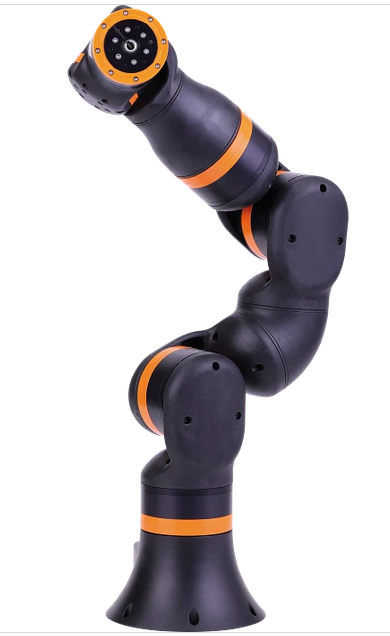
\includegraphics[width=0.3\textwidth]{chapter3_04.png}
    \captionsetup{width=1\linewidth}
    \caption{Igus ReBeL 6-DoF robotic arm}
    \label{fig:c3_img04}
\end{figure}

This robotic arm was the ideal choice for the project since the open-source control option allows the development of
the control software for the arm, based on ROS2 software packages. The lightweight and compact design made it suitable
for mounting on top of the SCOUT 2.0 robot, without affecting the robot's mobility and performance. 
The arm's easy installation and operation allows one to quickly set up the arm and start developing the control software
and perception algorithms for the project. The robotic arm is provided with its external power supply, but it can also be 
powered using batteries since it does not require a high current to operate. This feature is essential for the project,
as the robotic arm can be mounted on a mobile robot platform without relying on a power supply connected to the wall outlet.
The batteries used to power the robotic arm are placed on top of the mobile robot, as shown in \ref{fig:c3_img15}.

% Add the image of the robotic arm software
\begin{figure}[t]
    \centering
    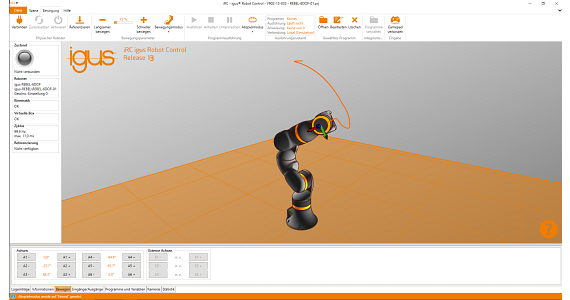
\includegraphics[width=0.8\textwidth]{chapter3_05.png}
    \captionsetup{width=1\linewidth}
    \caption{Igus ReBeL proprietary control software interface}
    \label{fig:c3_img05}
\end{figure}



\subsection*{Issues with Igus Rebel motors' encoders and calibration}

Due to the low-cost design of the ReBeL cobot, the arm's motors are equipped with encoders that are not as accurate
as the encoders used in more expensive metal-only robotic arms. This caused the arm's positioning accuracy to be lower than
the project's requirements, and the repeatability to be not good enough for the project's objectives.
The accuracy specified in the technical documentation of the arm is $\pm 0.1mm$, which is acceptable for the project's
needs, but the arm's actual accuracy was not as good as specified. Many tests were conducted to evaluate the arm's
end effector positioning accuracy, and the results showed that the error changes depending on the arm's configuration
and the height from the base of the arm's flange. The arm's accuracy is not consistent, and the repeatability
suffers from it. The tests showed also that the arm's accuracy is not dependent on the calibration of the arm's motors
but on the backlash and clearance of the gear components, which are not adjustable and cannot be calibrated.

A characteristic of the robotic arm's motors is that they have a certain amount of backlash and clearance,
which affects the amount of free movement of the arm's joints before the motor starts to move the joint.
This backlash and clearance in the gear components results also in the arm jiggling and vibrating when moving to a
different joint position, and not reaching the desired position with a smooth velocity profile.
Furthermore, the arm's internal gears are made of plastic, which is not as resilient and strong as metal gears.
This results in the arm suffering from its own weight, and the end effector moving a few centimeters down vertically from
the given pose when the end effector moves far away from the center of gravity of the robot's base. This is a critical
issue, as the position error does not depend linearly on the arm's configuration, and the arm's accuracy is not consistent
across the workspace. This characteristic of the robotic arm implies that an artificial compensation of the arm's
positioning error is necessary, to ensure that the arm's end effector reaches the desired position with higher precision,
even though the error cannot be completely eliminated.

\section{Sensors and Perception}

The mobile robot platform is equipped with several sensors, which are essential for the project's
objectives. The sensors used are perception systems that are used for mapping and localization, 
obstacle avoidance, object detection, and recognition.
Two main sensors are installed on the mobile manipulation robot: a 3D LiDAR sensor and an RGB-D stereo camera sensor.
The LiDAR sensor is in a fixed position, on top of the mobile robot base to have a 360° field of view, while the camera sensor
is mounted on the robotic arm's flange, allowing the camera to move with the arm's end effector.

\subsection{3D LiDAR}

The main sensor for environment perception for localization and navigation is mounted on top of the sensors
framework, a structure placed on top of T-slot rails that are bolted to the mobile robot's chassis.
The sensor is a \textit{Ouster OS1-64} LiDAR sensor, as shown in Figure \ref{fig:c3_img06}.
The OS1 offers clean, dense data across its entire field of view for accurate perception and crisp detail in industrial,
automotive, robotics, and mapping applications.
This sensor is a \textbf{64-plane LiDAR sensor}, capable of providing a 360-degree field of view with a range of $120$ meters. 
The sensor has a resolution of $\pm 0.1cm$ and a stable scan rate of $10 Hz$ at $1024$ points resolution.
The vertical and horizontal scan resolution are $\pm 0.01$°.
Its minimum range of $0.5$ meters makes it suitable for indoor environments, while its maximum range of $120$ meters
makes it suitable also for outdoor environments.
This sensor was employed to create maps of the environments and also to localize the robot within the environment.
It proved also useful for dynamic obstacle avoidance, thanks to its high resolution and scan rate.

%insert image of the LiDAR sensor
\begin{figure}[t]
    \centering
    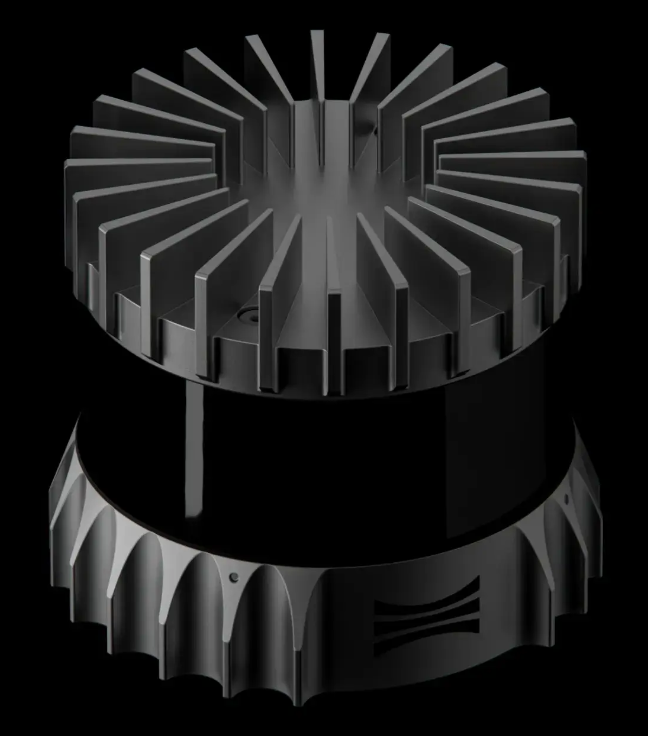
\includegraphics[width=0.5\textwidth]{chapter3_06.png}
    \captionsetup{width=1\linewidth}
    \caption{Ouster OS1-64 LiDAR sensor}
    \label{fig:c3_img06}
\end{figure}

\subsection{RGB-D Stereo Camera Sensor}

The robotic arm is equipped with a \textit{Intel Realsense D435} RGB-D stereo camera sensor, shown in Figure \ref{fig:c3_img07}.
The camera is mounted on the \textit{wrist} (the last joint link before the arm's flange) of the robotic arm,
allowing the camera to move with the arm's end effector.
The camera is used for object detection and recognition, and for ArUco markers detection and pose estimation.
This camera is chosen for this project because it is relatively cheap and provides both RGB and depth images,
which are essential for perception tasks in this robotic application.
The camera is also lightweight and compact, making it suitable for mounting on the cobot.

The Intel RealSense D435 is a stereo depth camera that is designed for capturing RGB and depth images.
The camera is equipped with a global shutter and a rolling shutter, which allows it to capture images with a resolution
of $1920\times1080$ pixels at $30$ frames per second. Throughout the development of the project,
the resolution of the Realsense camera was reduced to $640\times480$ pixels at $30$ frames per second. 
This allows for faster processing of the images since having a higher resolution would not benefit the perception
algorithms used in the project.
The camera has a field of view of $85.2$° horizontal, $58$° vertical,
and $94$° diagonal. The depth camera works within a range of $0.3$ meters to $3$ meters while maintaining 
high accuracy and precision.

% Add an image of the camera
\begin{figure}[t]
    \centering
    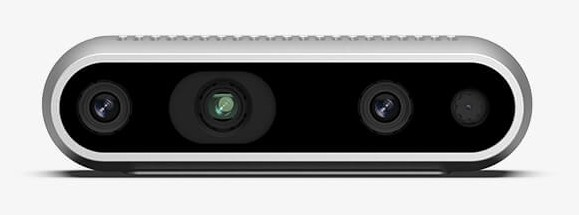
\includegraphics[width=0.5\textwidth]{chapter3_07.jpg}
    \captionsetup{width=1\linewidth}
    \caption{Intel RealSense D435 RGB-D stereo camera}
    \label{fig:c3_img07}
\end{figure}

\subsection{Intel Realsense Calibration}

For robotic applications employing perception sensors, it is essential to calibrate the sensors to provide accurate
and consistent data to the software. The calibration of the camera is necessary to correct the distortion
of the images and to provide accurate depth estimations from the depth sensor.
The calibration was fundamental for the correct development of the project, as the depth sensor employed was not
already calibrated by the manufacturer. This was a critical issue, as the depth sensor was used for many perception tasks.
Performing the calibration process enabled the camera to provide depth estimations consistent with the real-world distances
of the objects in the environment. It also enabled the estimation of the distance to the ArUco markers with high precision,
by using the correctly calibrated camera's intrinsic parameters. A test was conducted to measure the error of the camera's
depth sensor before and after the calibration process, and the results showed a significant improvement in the depth
estimations after the calibration process.

% Add the image of the calibration pattern
\begin{figure}[t]
    \centering
    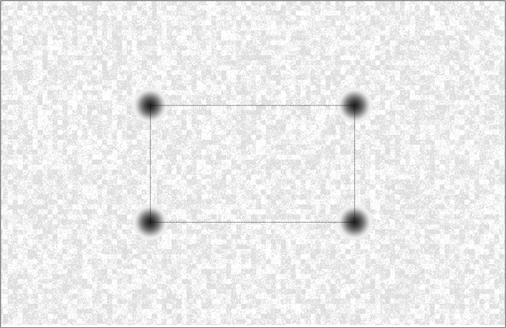
\includegraphics[width=0.5\textwidth]{chapter3_08.png}
    \captionsetup{width=1\linewidth}
    \caption{Calibration pattern used for the camera's depth image calibration}
    \label{fig:c3_img08}
\end{figure}


The calibration processes for the depth and image sensors was performed using the proprietary software provided by Intel:
\textit{Interl Realsense Self-Calibration Tool}, an application for \textbf{automatic on-chip calibration}.
This software allows to write the parameters for the sensors directly on the camera's EEPROM, ensuring that the calibration
parameters are stored on the camera and are not lost when the camera is disconnected from the computer.
The calibration process required many trials to find the best possible calibration parameters, but the results were
satisfactory. The process is quite straightforward as the software is completely automatic.
Two calibration procedures were carried out:

\begin{itemize}
    \item \textbf{Intrinsic parameters calibration}: this calibration process was used to calibrate the camera's 
    intrinsic parameters,
    such as the focal length, principal point, and distortion coefficients. This calibration was necessary to correct
    the distortion of the images and to provide accurate depth estimations from the RGB sensor. The calibration process
    required the camera to capture a series of images of a calibration pattern (checkerboard pattern) from different angles
    and distances. The calibration software then used these images to estimate the intrinsic parameters of the camera.
    \item \textbf{Depth sensor calibration}: this calibration process required the camera to capture a series of
    depth images of a calibration sheet, shown in Figure \ref{fig:c3_img08}, 
    which was a flat surface with known distances between the points.
    The calibration software then used these depth images to estimate the depth sensor's parameters, 
    such as the depth scale factor and the depth offset. 
    These parameters were necessary to correct the depth estimations of the camera's depth sensor.
\end{itemize}


After the calibration process, the camera's depth sensor was providing accurate and consistent depth estimations,
which were consistent with the real-world distances of the objects in the environment.

\section{Soft Gripper Actuator}

The robotic arm is equipped with a Soft Gripper Pneumatic Actuator from \textit{Soft Gripping}, depicted in Figure 
\ref{fig:c3_img09} while gripping an apple.
This gripper currently used for the project, is composed of three soft fingers, which are actuated by a pneumatic pump. 
Other versions of the gripper are available and provide two or more fingers. The fingers are made of
\textbf{silicone rubber}, which is soft and flexible, allowing the gripper to grasp and manipulate objects of different shapes
and sizes. The silicone material of the fingers is also non-slip, which ensures a secure grip on the objects.
The softness and flexibility of the silicone make it ideal for handling delicate and fragile objects.
The other advantage is that silicone is non-toxic and food-safe, making it suitable for handling products
in food industries.

% Add the image of the soft gripper
\begin{figure}[t]
    \centering
    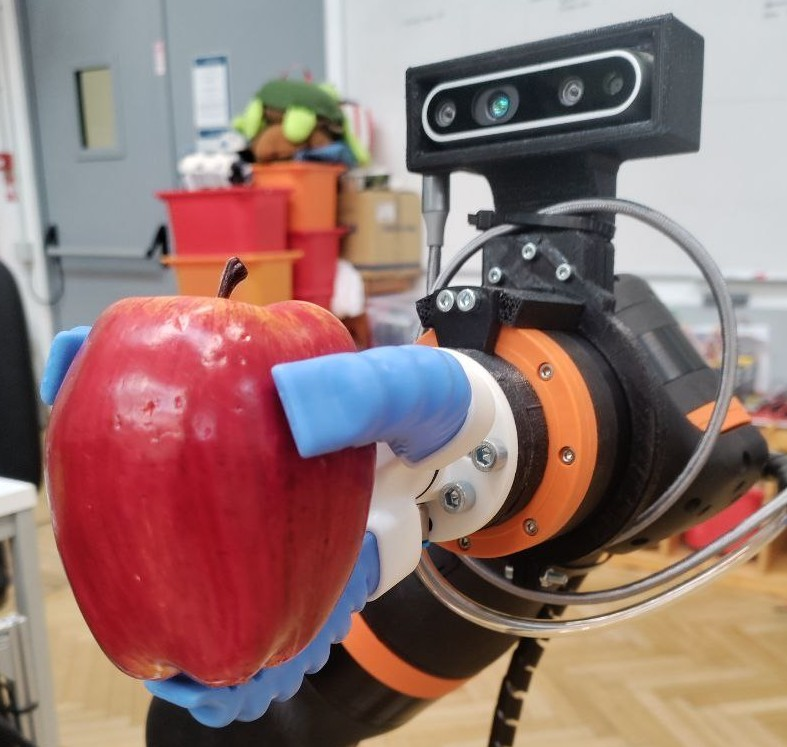
\includegraphics[width=0.6\textwidth]{c3_24.jpg}
    \captionsetup{width=1\linewidth}
    \caption{Soft Gripper Pneumatic Actuator handling an apple}
    \label{fig:c3_img09}
\end{figure}

The soft gripper is controlled by a pneumatic pump, shown in Figure \ref{fig:c3_img13}, 
which provides compressed air to the fingers, allowing them to open and close.
The pneumatic fingers can exist in three different states: they can be relaxed (i.e. not connected to the pneumatic pump),
opened when negative pressure is applied, and closed when positive pressure ($1$ bar) is applied.
The pneumatic pump that controls the soft gripper allows the user to set the pressure value used when closing the fingers,
using a valve. The pressure value cannot be changed dynamically via electronic control but is instead fixed and set manually.
Figure \ref{fig:sg_combined} shows the soft gripper mounted on the end effector
with the fingers opened and closed.

% Add a picture of the pneumatic pump
\begin{figure}[t]
    \centering
    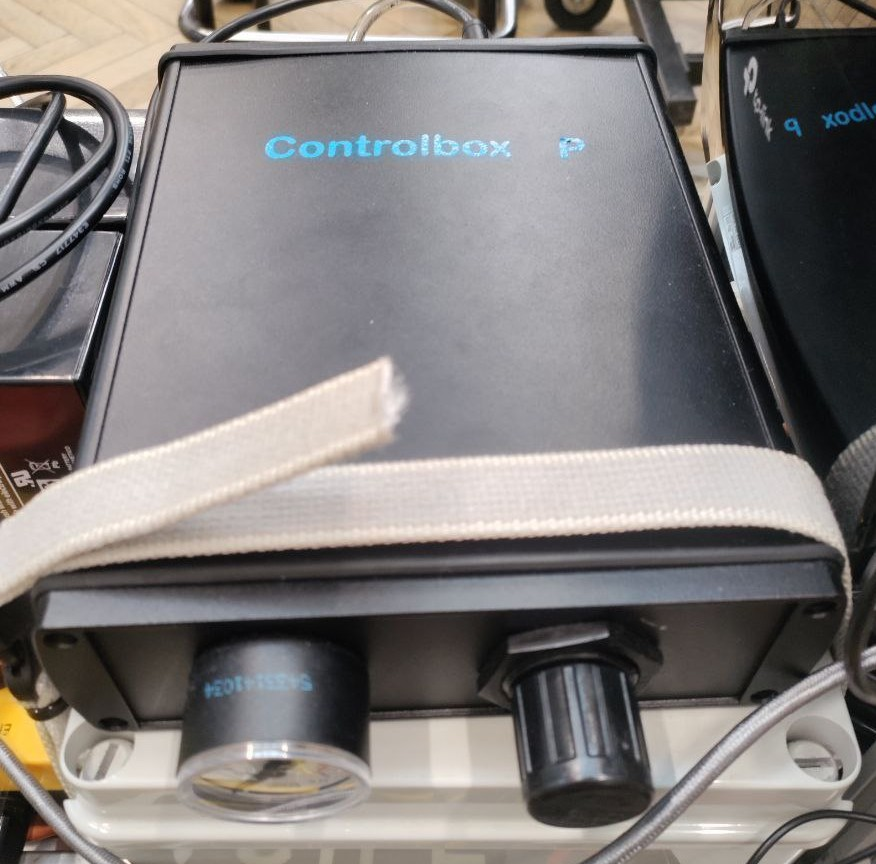
\includegraphics[width=0.6\textwidth]{c3_13.jpg}
    \captionsetup{width=1\linewidth}
    \caption{Pneumatic Pump control box secured on top of the mobile robot}
    \label{fig:c3_img13}
\end{figure}

The pneumatic pump provided with the soft gripper has only one output tube used for providing positive pressure
to the fingers, which closes them. The negative pressure for opening the fingers is instead provided by an internal valve,
that lowers the pressure compared to the atmospheric pressure. 
Other versions of the pneumatic pump provide also another output tube, which allows the user to control
the negative pressure value used when opening the fingers, but this feature requires an external vacuum compressor to work.

The gripper is mounted on the robotic arm's end effector, allowing the arm to grasp and manipulate
objects in the environment. It is placed close to the robotic arm's flange to ensure
that the mobility and reach of the end effector are not affected by the gripper's size.
Furthermore, the soft gripper is very lightweight and compact, making it suitable for mounting on the cobot.

% Add pictures of the gripper opened and closed
\begin{figure}[t]
    \centering
    \begin{subfigure}{0.45\textwidth}
        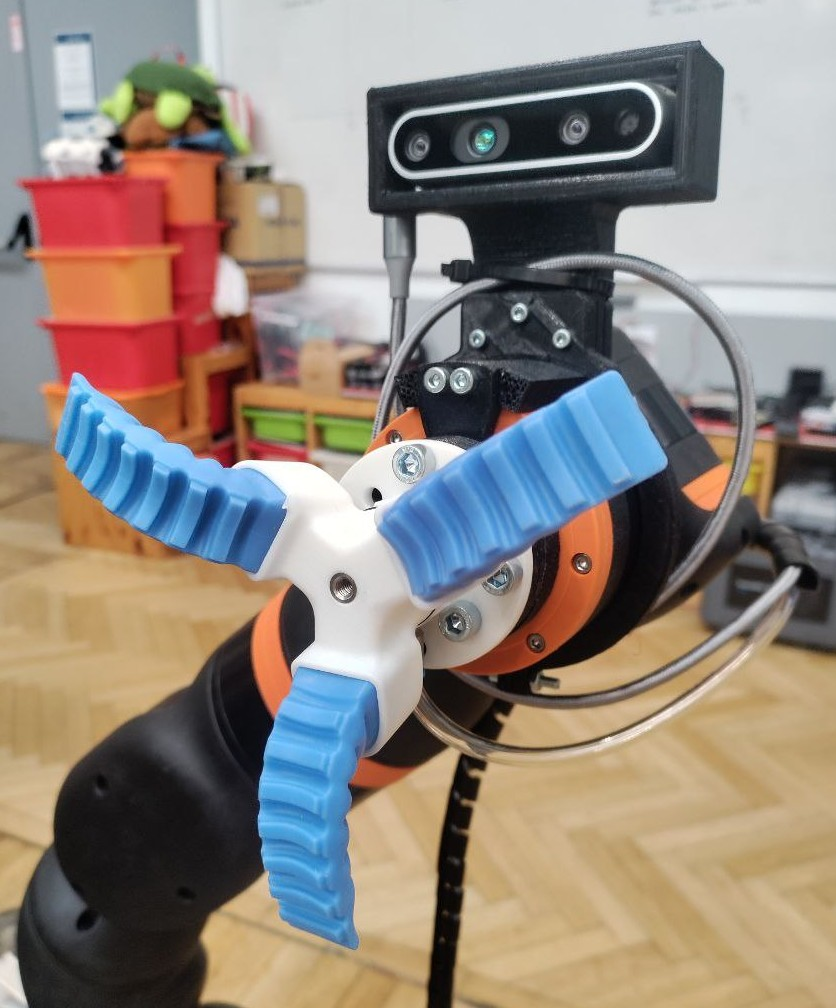
\includegraphics[width=1\textwidth]{c3_26.jpg}
        \caption{Soft Gripper opened}
        \label{fig:opened}
    \end{subfigure}
    \hfill % Optional: Adds space between images
    \begin{subfigure}{0.45\textwidth}
        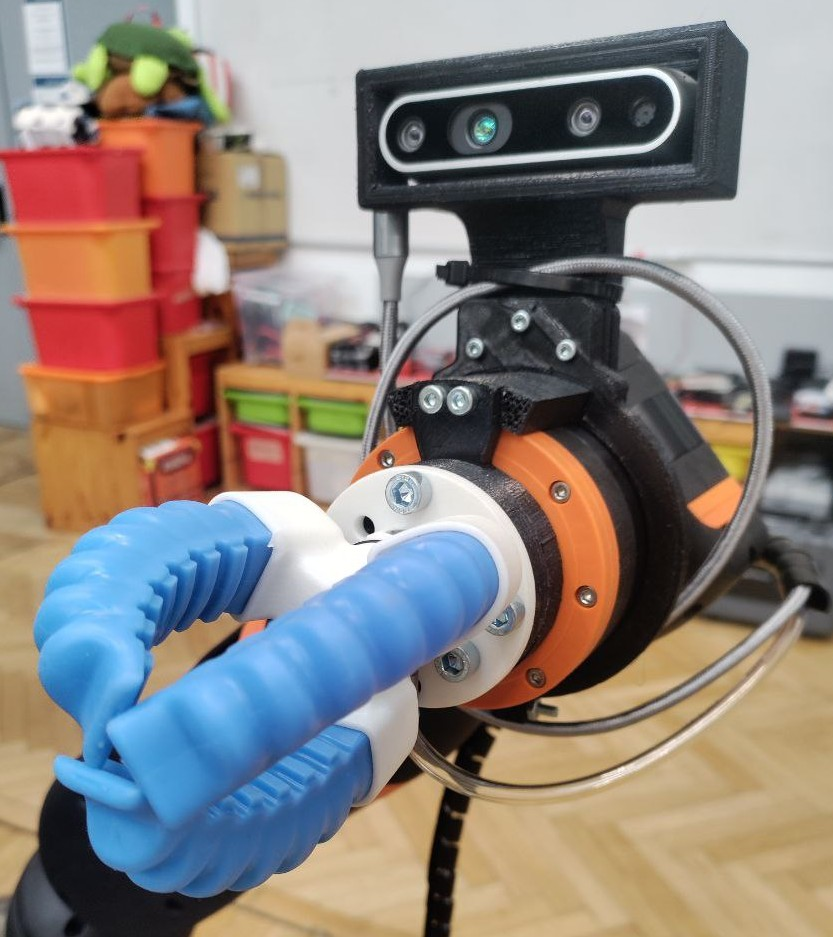
\includegraphics[width=1.07\textwidth]{c3_25.jpg}
        \caption{Soft Gripper closed}
        \label{fig:closed}
    \end{subfigure}
    \caption{Soft Gripper mounted on the end effector}
    \label{fig:sg_combined}
\end{figure}


The pump provides four digital pins for controlling its operation, which are used to open and close the fingers.
A simple system capable of controlling the pump's operation was created using an \textbf{Arduino UNO microcontroller}.
The Arduino UNO is connected to the robot's computer via USB, allowing the computer to send commands to the Arduino
via the serial port. The Arduino UNO is then connected to the pneumatic pump via a relay module,
composed of four different relays, each controlling a different digital pin of the pump. The relays were necessary
to provide an output voltage of $24$V, while the Arduino UNO provides only 5V via its digital pinout.
The relays are very inexpensive and fast in switching, allowing efficient
control of the pump's operation with the microcontroller's digital pin outputs.

The installation of the relays requires simple circuitry for the control system, so it can be easily positioned
on the mobile robot platform, without occupying much volume.
Figure \ref{fig:c3_img10} shows the Arduino UNO microcontroller and the relay module used to control the pneumatic pump,
installed on the mobile robot platform. Figure \ref{fig:pneumatic_circuit} shows the circuit diagram of the 
connections between the microcontroller and the pneumatic pump digital pinout. In the circuit diagram,
the Arduino UNO digital pins are connected to the relay module and provide the input switch for the relays.
The relays are then connected to the pneumatic pump's digital pins, which control the pump's operation.
All relays are connected to the same ground and power supply of the Arduino UNO.

% Add a picture of the Arduino UNO and the relay module
\begin{figure}[t]
    \centering
    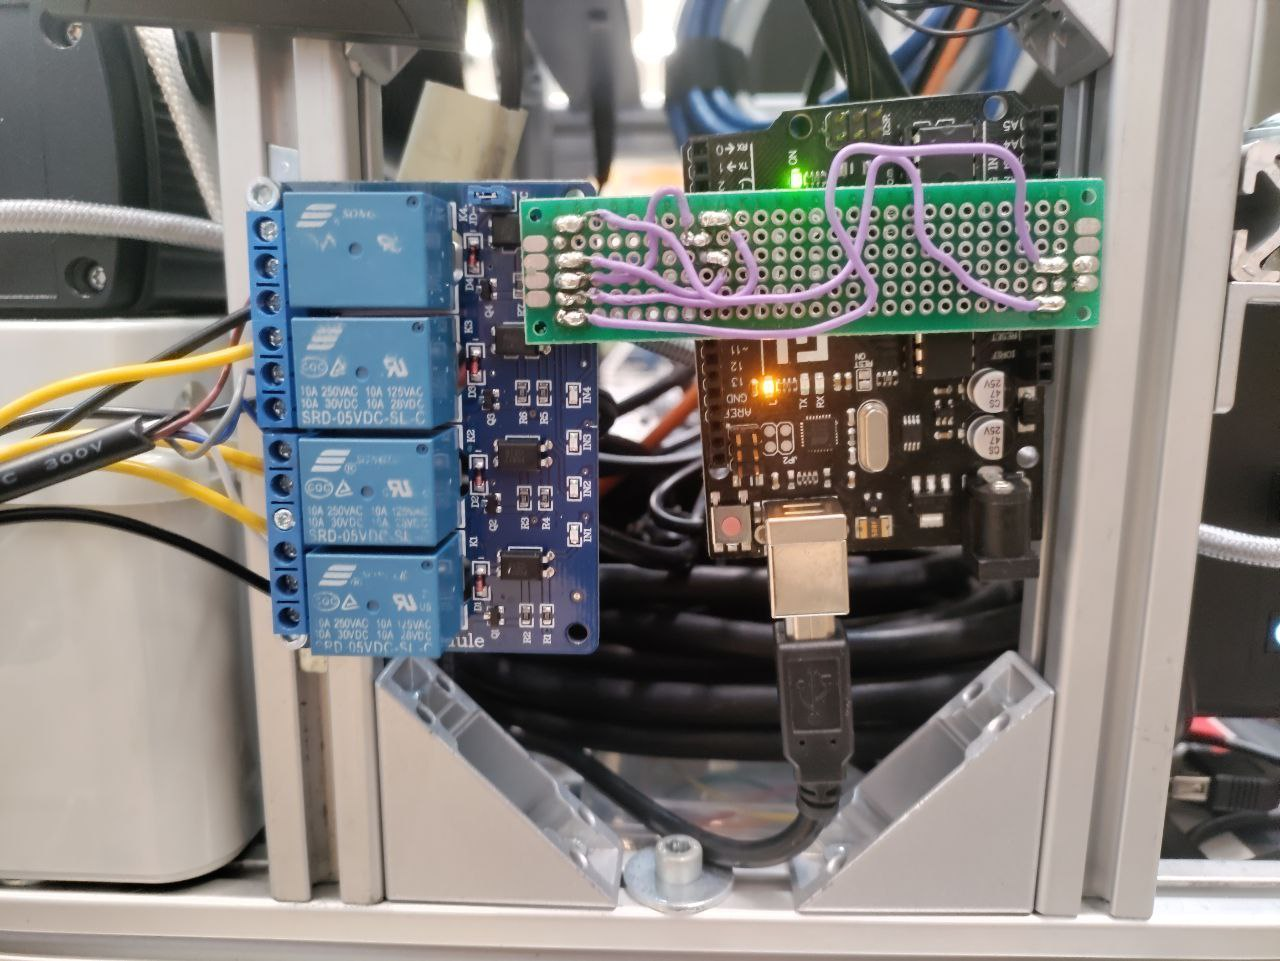
\includegraphics[width=0.6\textwidth]{c3_11.jpg}
    \captionsetup{width=1\linewidth}
    \caption{Arduino UNO microcontroller and relay module used to control the pneumatic pump.}
    \label{fig:c3_img10}
\end{figure}

\begin{figure}[t]
    \centering
    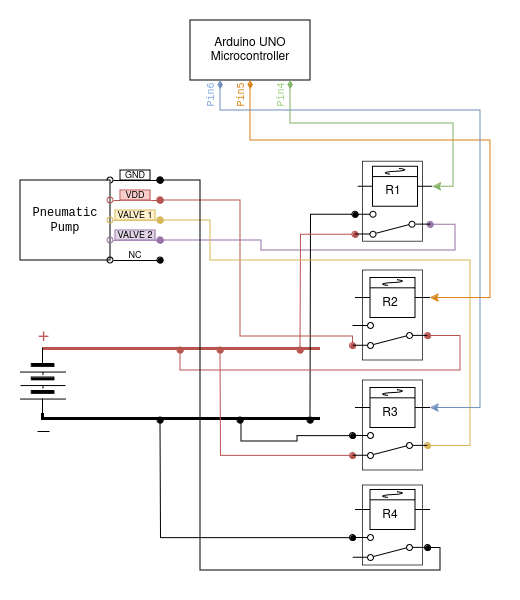
\includegraphics[width=0.6\textwidth]{pneumatic_circuit.png}
    \captionsetup{width=1\linewidth}
    \caption{Circtuit schematic for the pneumatic pump control system using an Arduino UNO and relay modules.}
    \label{fig:pneumatic_circuit}
\end{figure}

\section{3D Printed Mounts Design}

Mounting the sensors and electronic devices on the mobile robot platform required the design and 3D printing
of custom mounts. The mounts were designed using the \textit{Fusion 360} CAD software, which allowed me to create
precise and accurate models of the mounts. The mounts were then 3D printed using the laboratory's 3D printer,
which is a \textit{Creality CR-10S} 3D printer. The 3D printer employs the Fused Deposition Modeling (FDM) technique,
which uses a thermoplastic filament to create the 3D models layer by layer. The material of choice
for the 3D prints was \textit{PETG} (Polyethylene Terephthalate Glycol), which is a strong and durable material,
suitable for mechanical parts and mounts. The PETG material is also resistant to mechanical stress and heat,
making it the ideal material for the mounts for these kinds of applications.

Two versions of the mount were designed and printed for the cobot's flange:

\begin{itemize}
    \item \textit{Mount V1} \ref{fig:mountv1}: a mount for the Realsense camera and a digital button on top of a cylinder used
    for pressing buttons on a control panel. The mount was designed to be robust and easy to switch with other
    mount extensions. This mount was used for the first demos and tests of the project.
    \item \textit{Mount V2} \ref{fig:mountv2}: a mount for the Realsense camera and the soft gripper as an end-effector.
    This mount was designed to be compact, robust, and more effective for the final versions of the project.
\end{itemize}

The 3D-printed mounts were designed to be lightweight and compact, to ensure that the robot's mobility and stability
were not affected. The mounts were also designed to be robust and durable, to withstand the vibrations and shocks
of the mobile robot platform. The mounts are designed to be
mounted with several screws and bolts, ensuring that the sensors and electronic devices are securely attached to the robot.
These mounts demonstrated to be very effective and reliable, as they withstood the vibrations while maintaining
the sensors in their fixed position.

\subsection{MountV1}

% Add pictures of the Mount V1 render and 3D print
\begin{figure}
    \centering
    \begin{subfigure}{\textwidth}
        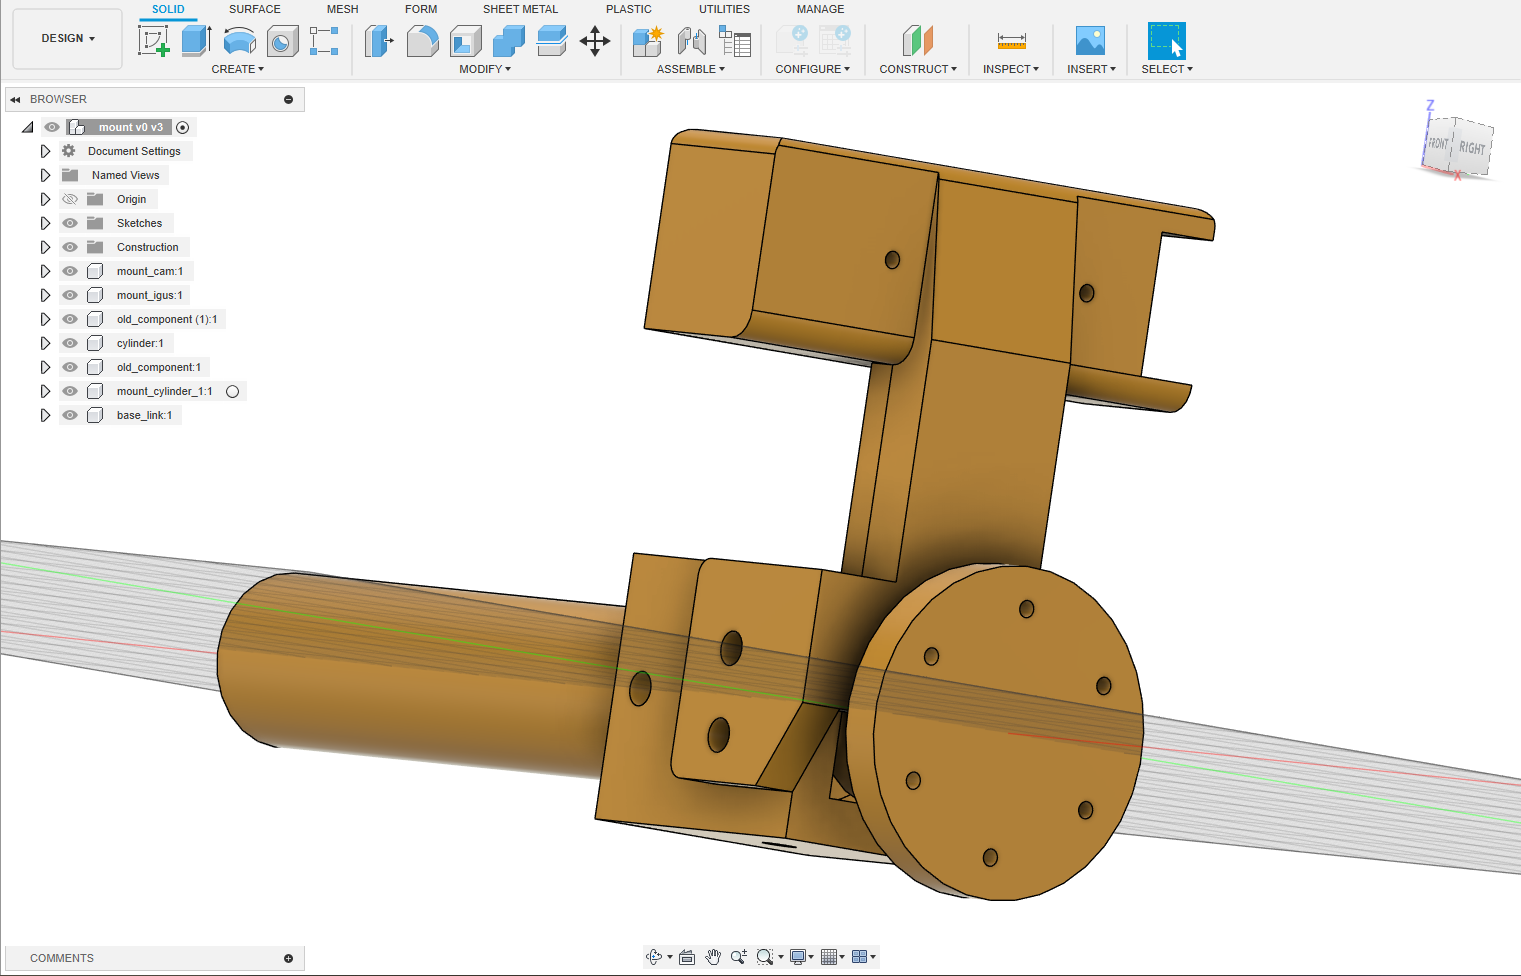
\includegraphics[width=0.9\textwidth]{c3_20.png} % Replace with your image file
        \caption{Back side view of the 3D design}
        \label{fig:frontv1}
    \end{subfigure}
    
    \vspace{1em} % Add some vertical space between images (adjust as needed)

    \begin{subfigure}{\textwidth}
        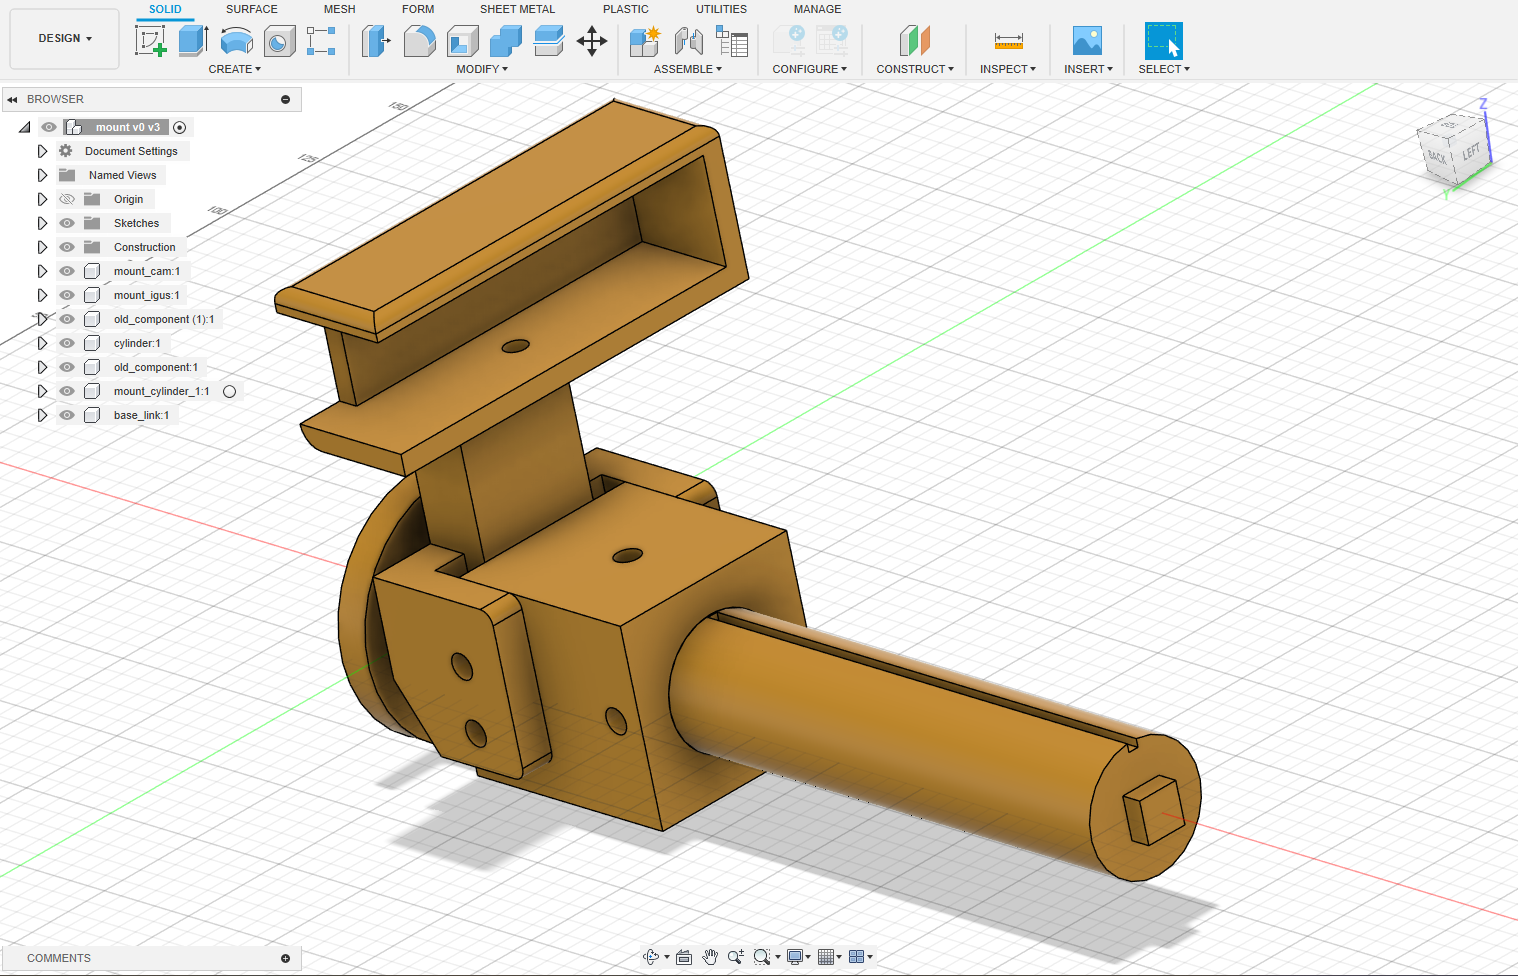
\includegraphics[width=0.9\textwidth]{c3_23.png} % Replace with your image file
        \caption{Frontal side view of the 3D design}
        \label{fig:sidev1}
    \end{subfigure}

    \caption{MountV1 Design screenshots from \textit{Autodesk Fusion 360}}
    \label{fig:mountv1}
\end{figure}

The first version of the mount, alias \textit{Mount V1}, shown in Figure \ref{fig:mountv1},
was designed to be robust and allow to switch easily the mount extensions. 
MountV1 is lightweight and the cylinder placed on it is long enough to ensure that the cobot's end effector
would be able to reach objects not in the immediate vicinity of the robot. The mount is also
compact, with the stereo camera mounted in front of the cobot's flange, and the digital button mounted on top
of a cylinder used for pressing buttons on a control panel. The 3D print resulted in a very robust and durable
structure.

After many tests, the cylinder was then shrunk to a smaller length, to ensure that the cobot's end effector
mobility was not affected negatively. This allowed the cobot's end effector to reach objects
in the vicinity with fewer limitations and constraints on its orientation, at the expense of a slightly reduced reach.
The digital button mounted on the extremity of the end effector
was initially used as a digital feedback mechanism for the pressure
of the buttons on the control panel. This button was later removed, as it was not necessary for the project's
objectives. The mount was then used for the first demos and tests of the project, and it proved to be very effective.

One of the main issues encountered with the mount was the \textbf{reduced field of view of the stereo camera}, due to its
installation on the cobot's flange. The camera was placed at about $7$ cm from the center of the cobot's flange,
making it possible for the camera's field of view not to be obstructed by the cylinder,
while maintaining the mount compact.
Many tests and applications showed that the best configuration would be to mount the camera on top of the wrist,
to enlarge the field of view. MountV1 was used for the first applications but then replaced with an
improved version for the following activities.

\subsection{MountV2}

% Add pictures of the Mount V2 render and 3D print
\begin{figure}
    \centering

    \begin{subfigure}{\textwidth}
        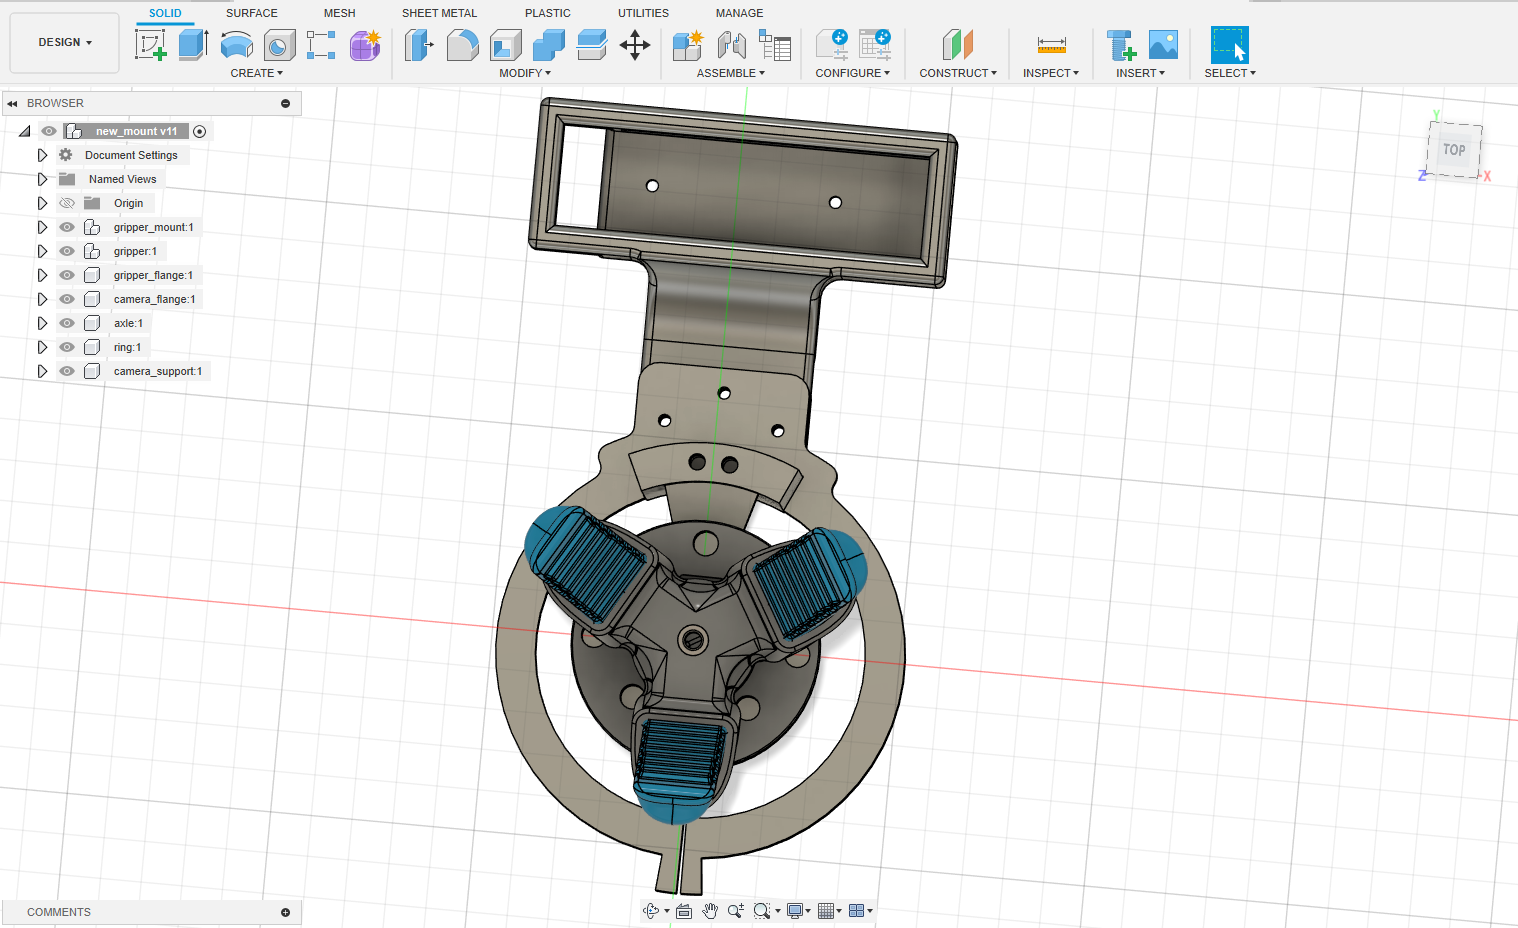
\includegraphics[width=\textwidth]{c3_21.png} % Replace with your image file
        \caption{Front view of the 3D design}
        \label{fig:frontv2}
    \end{subfigure}
    
    \vspace{1em} % Add some vertical space between images (adjust as needed)

    \begin{subfigure}{\textwidth}
        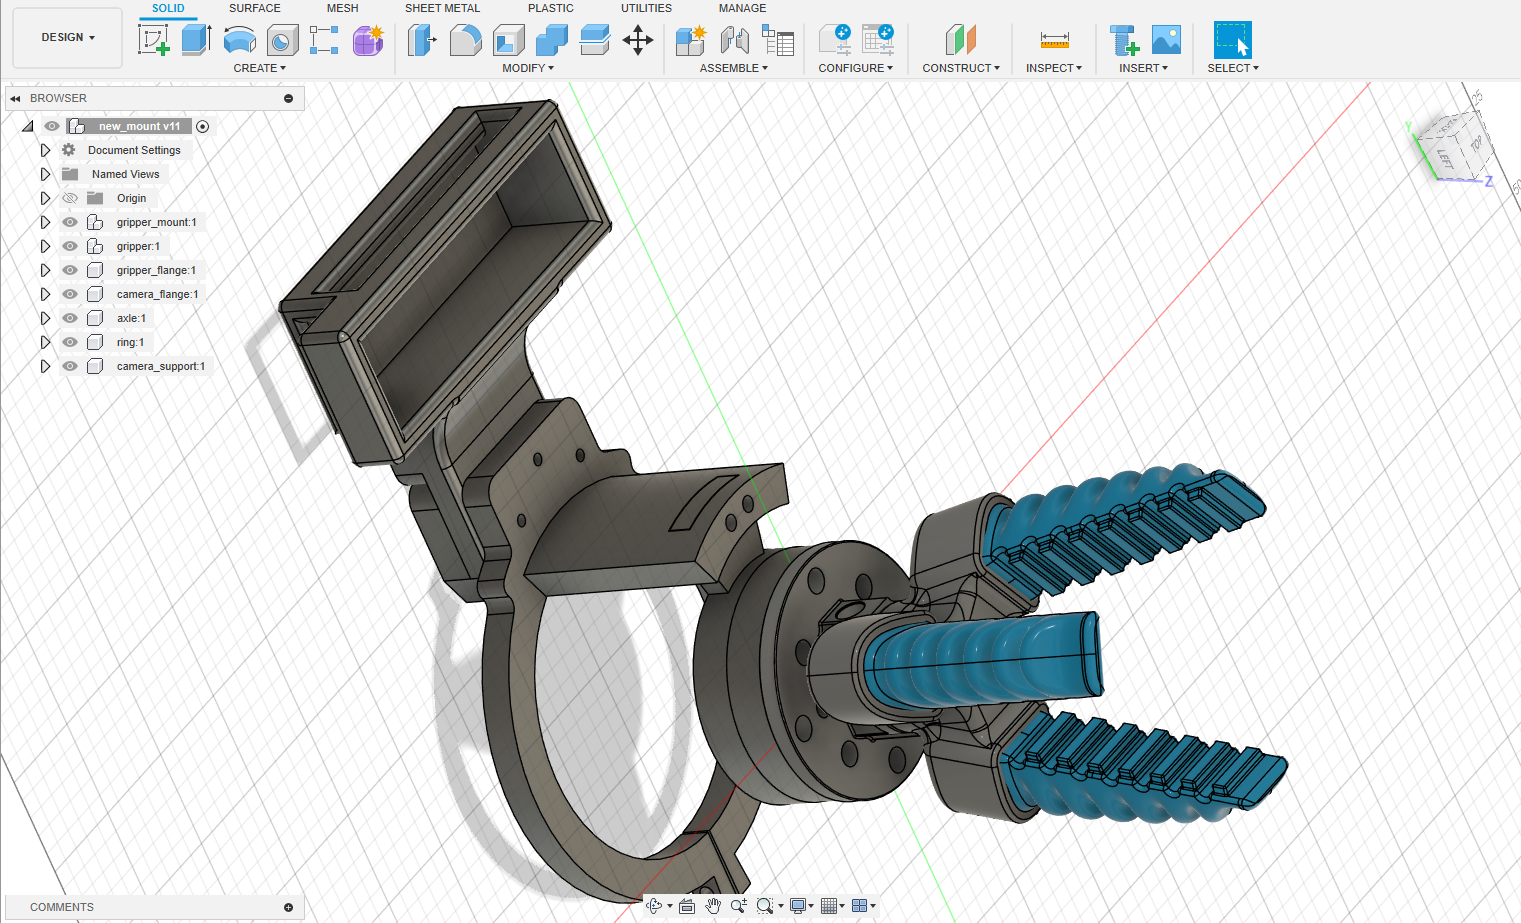
\includegraphics[width=\textwidth]{c3_24.png} % Replace with your image file
        \caption{Side view of the 3D design}
        \label{fig:sidev2}
    \end{subfigure}

    \caption{MountV2 Design screenshots from \textit{Autodesk Fusion 360}}
    \label{fig:mountv2}
\end{figure}

The second version of the mount, alias \textit{Mount V2}, was designed to be compact, robust, and more effective
for the agricultural applications of the project. The mount,
shown in Figure \ref{fig:mountv2}, comprises three parts:
the flange connector, the camera mount, and the soft gripper mount. The system is composed of multiple components,
each individually 3d printed, to ensure an efficient printing process that allows printing the components separately
if they break or get damaged. This was an important feature, considering that each component was redesigned multiple
times after failed prints or design inefficiencies.

The \textbf{soft gripper mount} is used to mount the soft gripper on the cobot's flange connector, allowing the cobot's
end effector to grasp and manipulate objects in the environment.
The \textbf{flange connector} is used to connect the mount to the cobot's flange, ensuring that the mount is securely 
attached using screws. The flange connector was designed to be lightweight and compact, 
to ensure that the 3d printing process would be fast and structurally sound. This piece is also
robust and durable, to withstand the vibrations and shocks of the cobot's movements.
The \textbf{camera mount} is used to mount the stereo camera on top of the cobot's wrist,
ensuring that the camera has a wider field of view compared to its previous version.
The camera mount is designed to be attached to the flange connector on the cobot's wrist with screws and bolts,
ensuring that the camera is securely attached to the cobot while preventing vibrations that could
offset the sensor position and orientation. The camera mount hosts the camera cable angled connector.
This angled connector is magnetic, and it prevents the cable from being pulled out of the camera when
the cobot's end effector moves around. This was a critical feature, set to avoid the camera's cable
being broken or damaging the internal USB-C port of the stereo camera. The MountV2 installed on the cobot
is shown in \ref{fig:c3_img17}.

\begin{figure}[t]
    \centering
    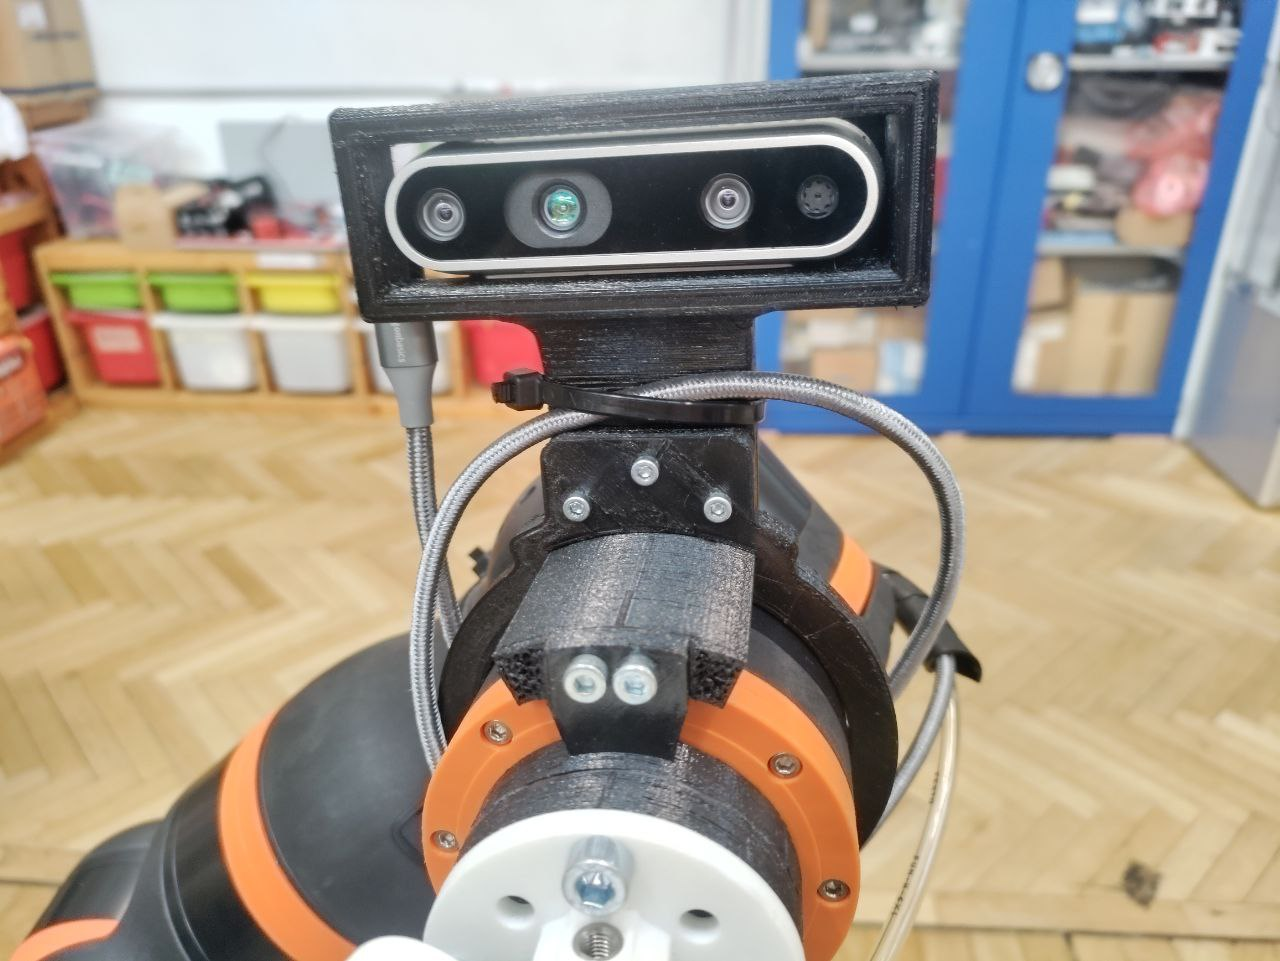
\includegraphics[width=0.6\textwidth]{c3_17.jpg}
    \captionsetup{width=1\linewidth}
    \caption{3d-printed mountV2 on the arm's wrist}
    \label{fig:c3_img17}
\end{figure}

\subsection{GPS Antenna Support}

Another mount was designed and created: the \textbf{mount for the GPS antenna}, which was used for outdoor localization
and navigation tasks. The GPS antenna mount was designed to be placed on top of the LiDAR sensor, ensuring
that the antenna had a clear view of the sky and the satellites. The mount was also designed to be lightweight
and quick to install, without affecting the LiDAR sensor's field of view, and without using any screws or bolts.
Figure \ref{fig:gpsprint} shows the mount installation on top of the LiDAR sensor, while Figure \ref{fig:gps3d}
shows the 3D design of the mount.
While the GPS was not used directly in this project, the mount was part of a general redesign of the mobile robot platform,
specifically the sensor framework support structure. The redesign was necessary to install the robotic arm and achieve
a mobile manipulator configuration while moving the GPS to a location that does not impede the movement of the arm.

% Add pictures of the GPS antenna mount render and 3D print
\begin{figure}[t]
    \centering
    \begin{subfigure}{0.3\textwidth}
        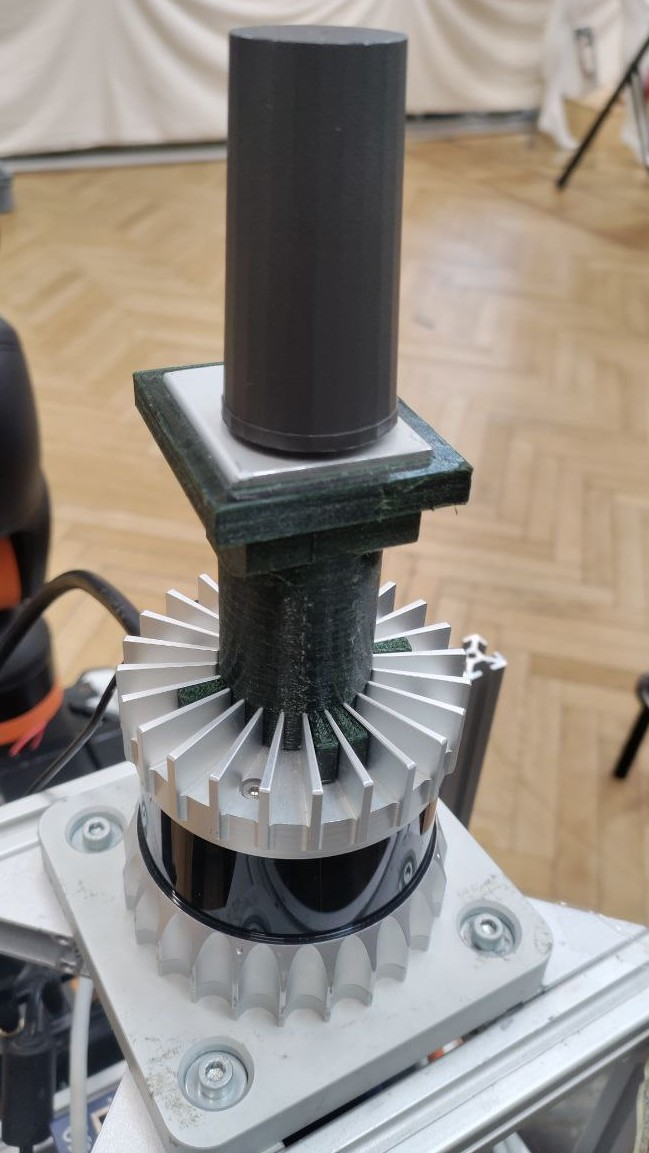
\includegraphics[width=0.7\textwidth]{c3_20.jpg}
        \captionsetup{width=0.9\linewidth}
        \caption{GPS antenna 3D printed mount}
        \label{fig:gps3d}
    \end{subfigure}
    \hfill
    \begin{subfigure}{0.67\textwidth}
        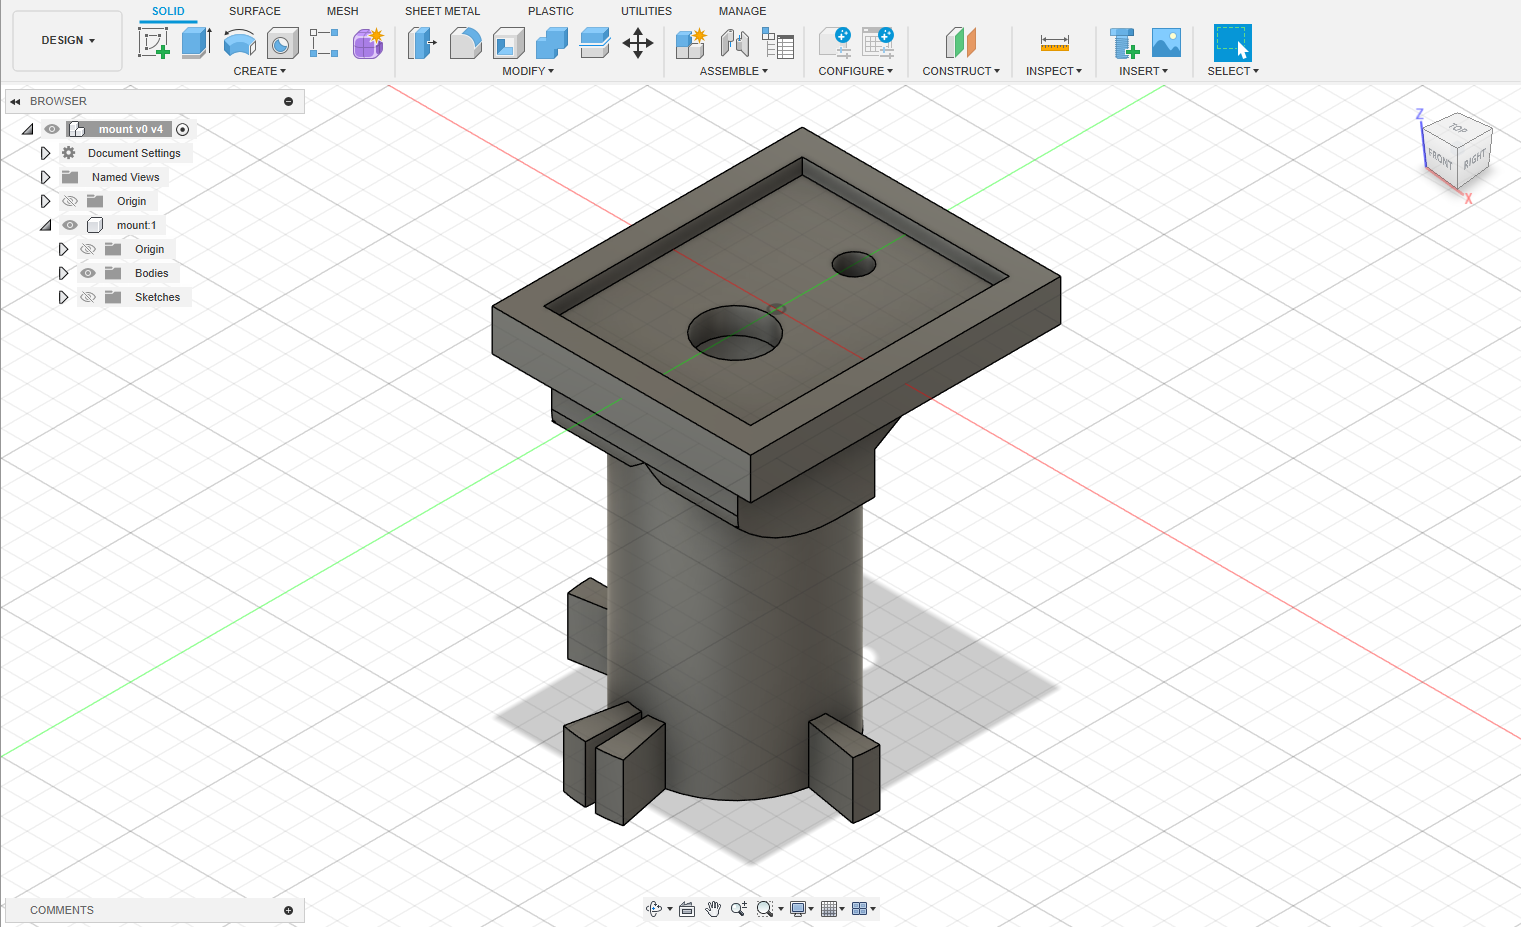
\includegraphics[width=1.0\textwidth]{c3_22.png}
        \caption{3D design}
        \label{fig:gpsprint}
    \end{subfigure}
    \captionsetup{width=1\linewidth}
    \caption{GPS antenna mount design and 3D-print on top of the LiDAR}
    \label{fig:c3_gps}
\end{figure}

\subsection{3D printer maintenance and configuration}

The AIRLab's 3D printer is a valuable resource for researchers and students, and achieving high-quality prints
requires specific conditions. In order to optimize the 3d printing results and meet these quality standards,
a series of maintenance and calibration procedures were undertaken to address issues such as 
\textbf{stringing and under-extrusion}, which significantly impacted the quality of 3D printed objects.
The printer's bed was calibrated, to ensure that the prints were of high quality and accurate.
The nozzle was substituted with a new one, and the hot end was unclogged, to ensure that the filament could extrude correctly
and with the best flow. Cleaning the printer's bed and the extruder proved to be useful too, and ensured
that the prints were sticking correctly to the bed while avoiding the warping of the prints.
After these maintenance operations, the printer was working correctly, and the prints were of higher quality.

\section{Batteries and Power Management}

The mobile robot's internal battery is capable of powering all the onboard sensors and computational
units. To meet the specific voltage and current requirements of these devices, 
two DC/DC converters are employed, one of which is shown in Figure \ref{fig:c3_img03}:

\begin{itemize}
    \item one DC/DC converter with an output voltage of 12V at a maximum of 15A for the on-board computer, router, and switch
    \item one DC/DC converter with an output voltage of 24V at a maximum of 5A for the LiDAR.
\end{itemize}

The mobile robot platform's internal batteries are not sufficient to power the robotic arm and the pneumatic pump
mounted on board. To power these devices, an external power supply is used, which provides 24V at a maximum of 10A.
The cobot is powered by two 12V \textbf{lead batteries} \ref{fig:c3_img15} with 9Ah of power capacity, 
which provides the necessary power to the robotic arm motors and the pneumatic pump. 
The batteries are mounted and secured on the robot's base,
ensuring that the robot is powered and operational during its missions. There are two battery packs available,
which can be switched easily when one of them is discharged.

% Add a picture of the batteries
\begin{figure}[t]
    \centering
    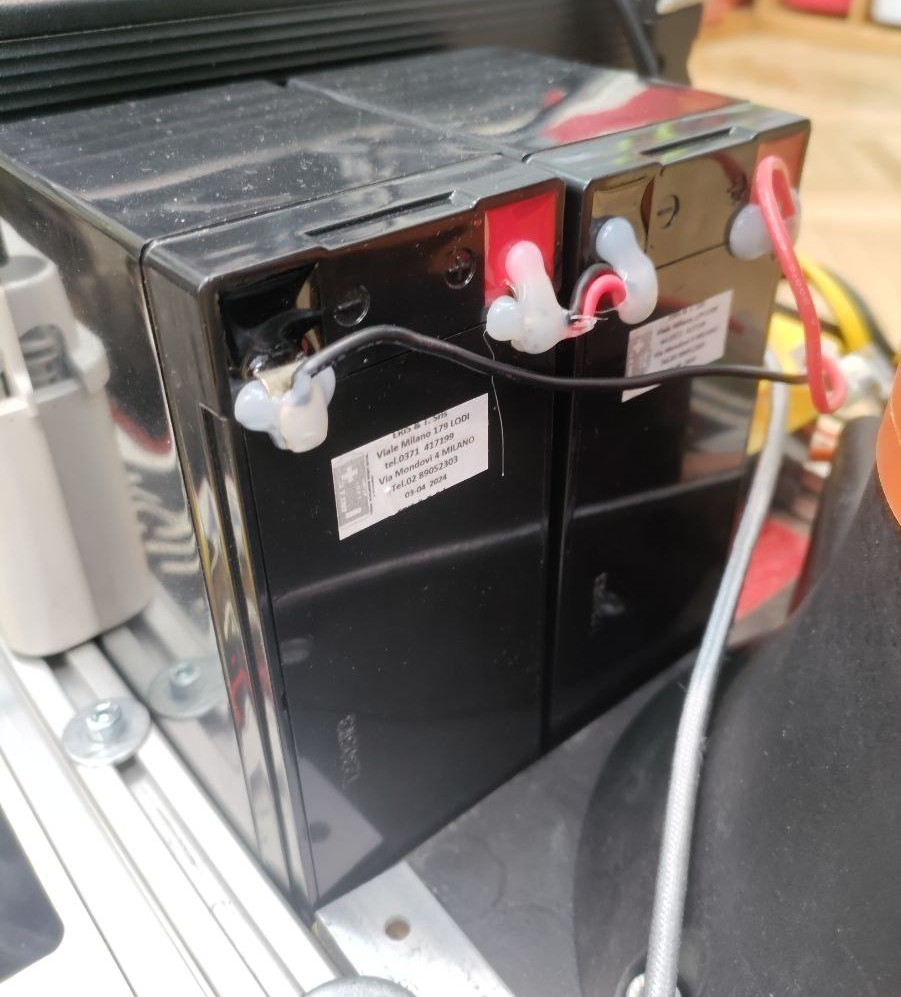
\includegraphics[width=0.5\textwidth]{c3_15.jpg}
    \captionsetup{width=1\linewidth}
    \caption{Lead batteries mounted onboard for the cobot and pneumatic pump}
    \label{fig:c3_img15}
\end{figure}

% Add image of DC/DC converters
\begin{figure}[t]
    \centering
    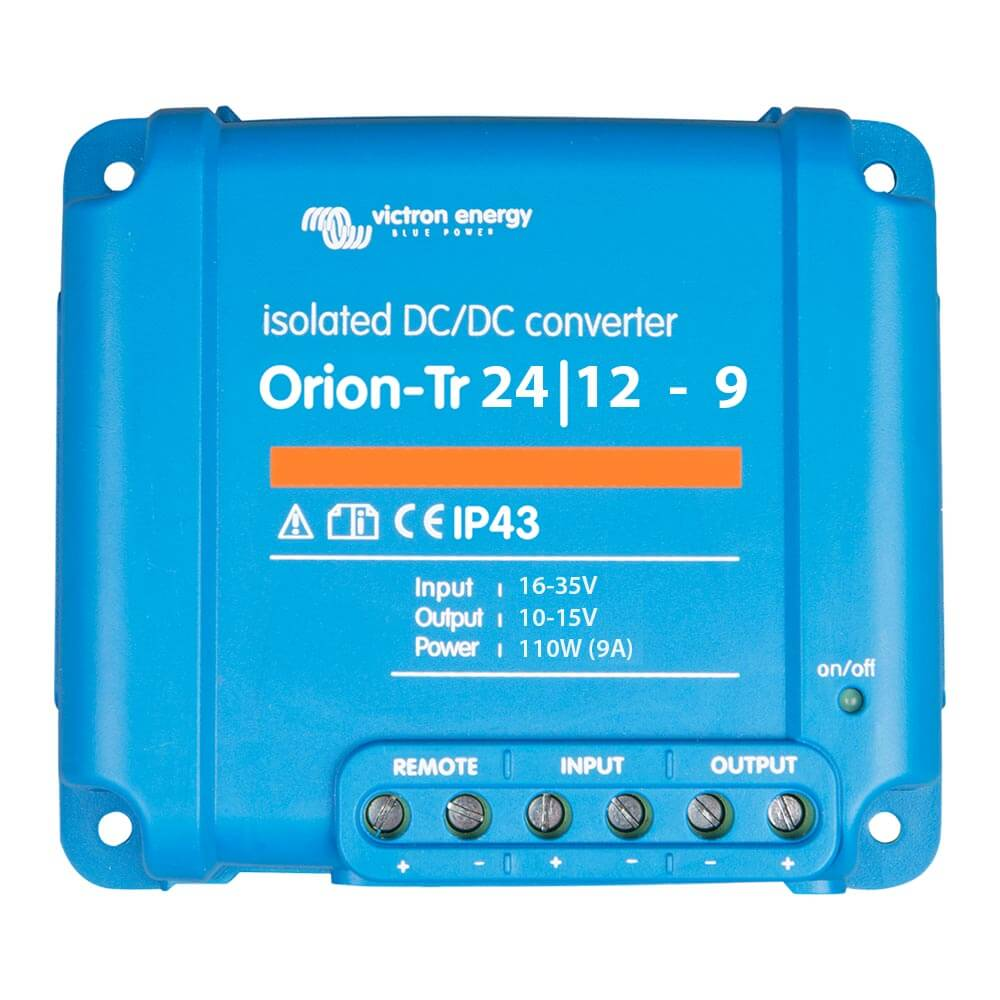
\includegraphics[width=0.4\textwidth]{chapter3_03.jpg}
    \captionsetup{width=1\linewidth}
    \caption{DC/DC converter used to power the robot's sensors and computer}
    \label{fig:c3_img03}
\end{figure}

The pneumatic pump requires an external power supply, hence it was necessary to provide power via
the \textbf{onboard batteries}.
The pneumatic pump must be controlled at $24$V, as the pump's solenoid valve requires this voltage to operate.
The pump is powered by a $24$V lead battery, which is the same battery powering
the robotic arm. It was necessary to create a system for powering both the robotic arm and the pneumatic pump
with the same batteries, due to the limited space available on top of the mobile robot platform.
A convenient and cheap solution found is to use Molex cables and connectors that connect both the cobot
and the pump to the same battery pack.
These Molex cables proved to be a reliable and optimal solution, as they allow to switch easily and quickly
between the onboard batteries and the external cobot power supply.
The Molex cable management is shown in \ref{fig:c3_img12}.

The cobot's proprietary power supply provides $24$V at a maximum of $10$A, which is enough to power the robotic arm
and the pneumatic pump simultaneously, since the pneumatic pump doesn't require a high current to operate.
The output connector of the external power supply is also a Molex cable, so that's why Molex connectors and cables
were used to connect the robotic arm and the pneumatic pump to the power systems. Both the batteries and the 
external power supply make use of the same connectors to power the cobot and the pneumatic pump.

% Add a picture of the Molex connectors and cables
\begin{figure}[t]
    \centering
    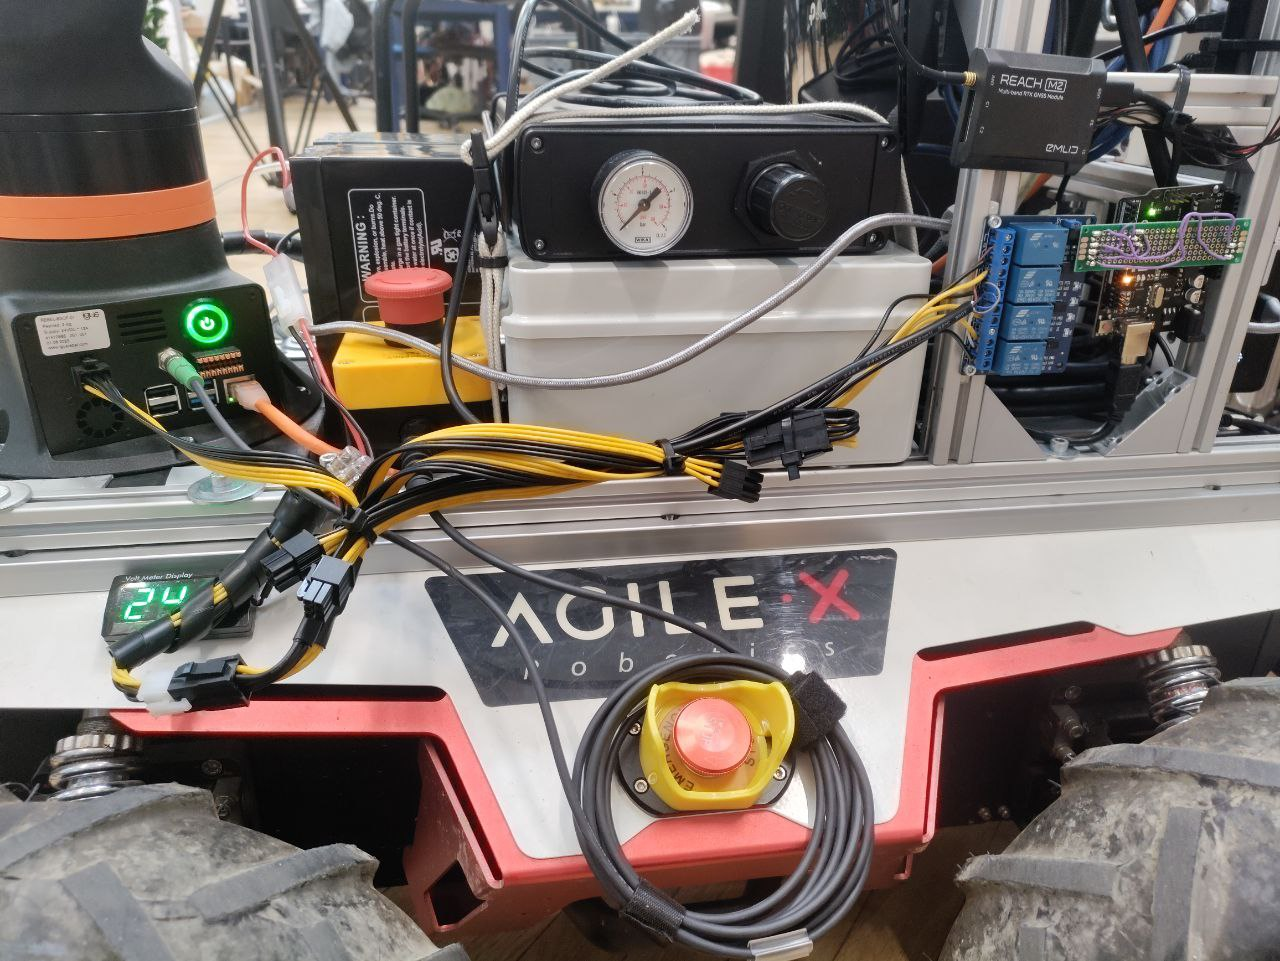
\includegraphics[width=0.6\textwidth]{c3_12.jpg}
    \captionsetup{width=1\linewidth}
    \caption{Molex connectors and power management for the cobot, pump, and relays}
    \label{fig:c3_img12}
\end{figure}

% Another tool used to power the robot is a \textit{Santino}, a Holy Figure card presenting \textit{Saint Staianet}, 
% the patron saint and protector of the mobile manipulation robot. This figure, placed in the front,
% as shown in Figure \ref{fig:c3_img19},
% helps and protects the robot during development and testing, ensuring everything
% works fine and smoothly. The Santino was also used to provide spiritual and religious guidance,
% ensuring the robot was blessed and protected during its missions.

% \begin{figure}[t]
%     \centering
%     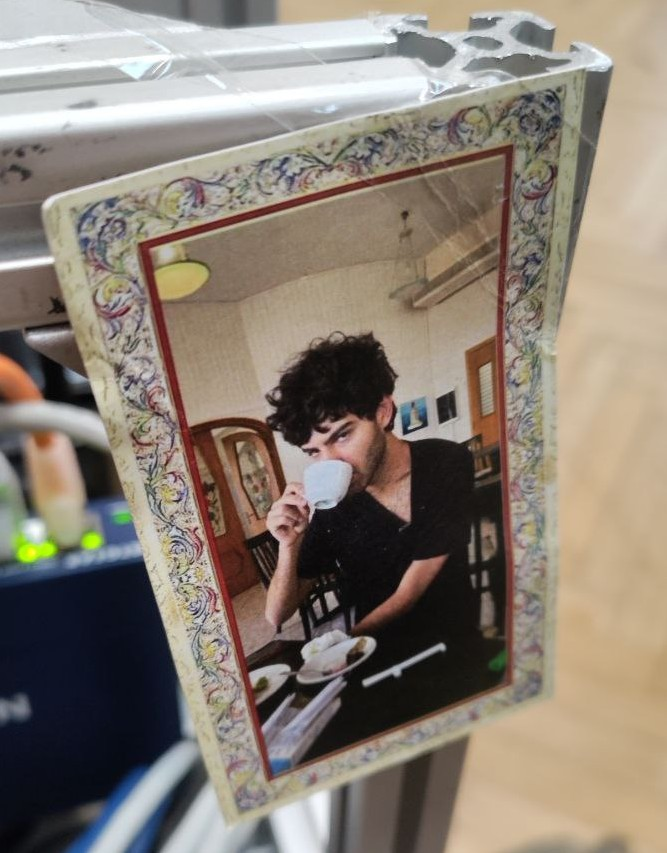
\includegraphics[width=0.5\textwidth]{c3_19.jpg}
%     \captionsetup{width=1\linewidth}
%     \caption{Santino}.
%     \label{fig:c3_img19}
% \end{figure}

\section{Mobile Manipulation Setup}

Figures \ref{fig:c3_img28} and \ref{fig:c3_img29} show the complete mobile manipulation setup, with the robotic arm
mounted on top of the Scout robot, and the soft gripper mounted on the robotic arm's end effector.
The setup shown in the figures is ready for the "soft grasping" demos, where the robot is tasked with grasping
and manipulating objects in simulated agricultural environments.

\begin{figure}[t]
    \centering
    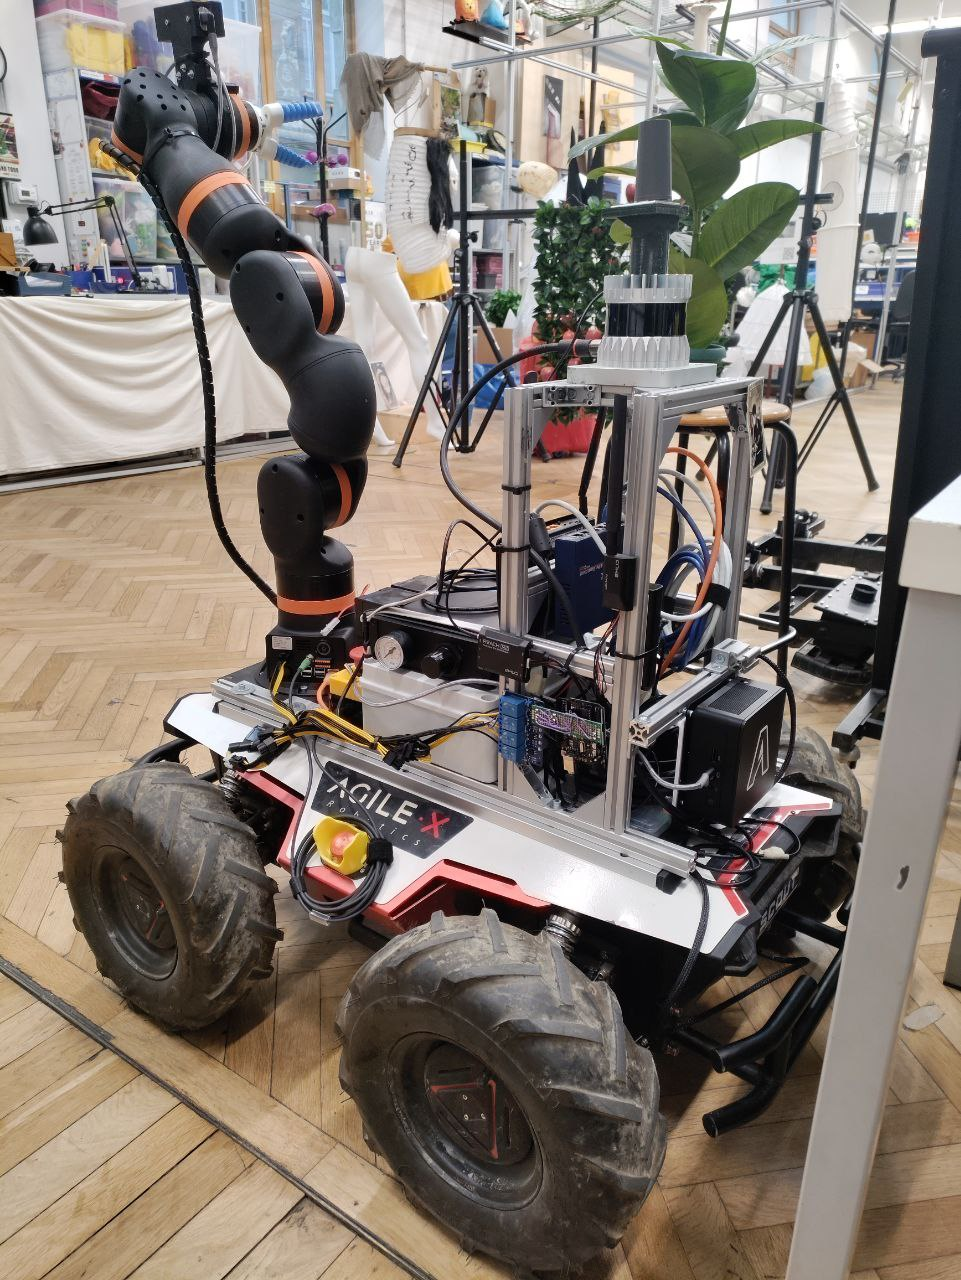
\includegraphics[width=0.8\textwidth]{c3_29.jpg}
    \captionsetup{width=1\linewidth}
    \caption{Lateral view of the robots}
    \label{fig:c3_img29}
\end{figure}

\begin{figure}[t]
    \centering
    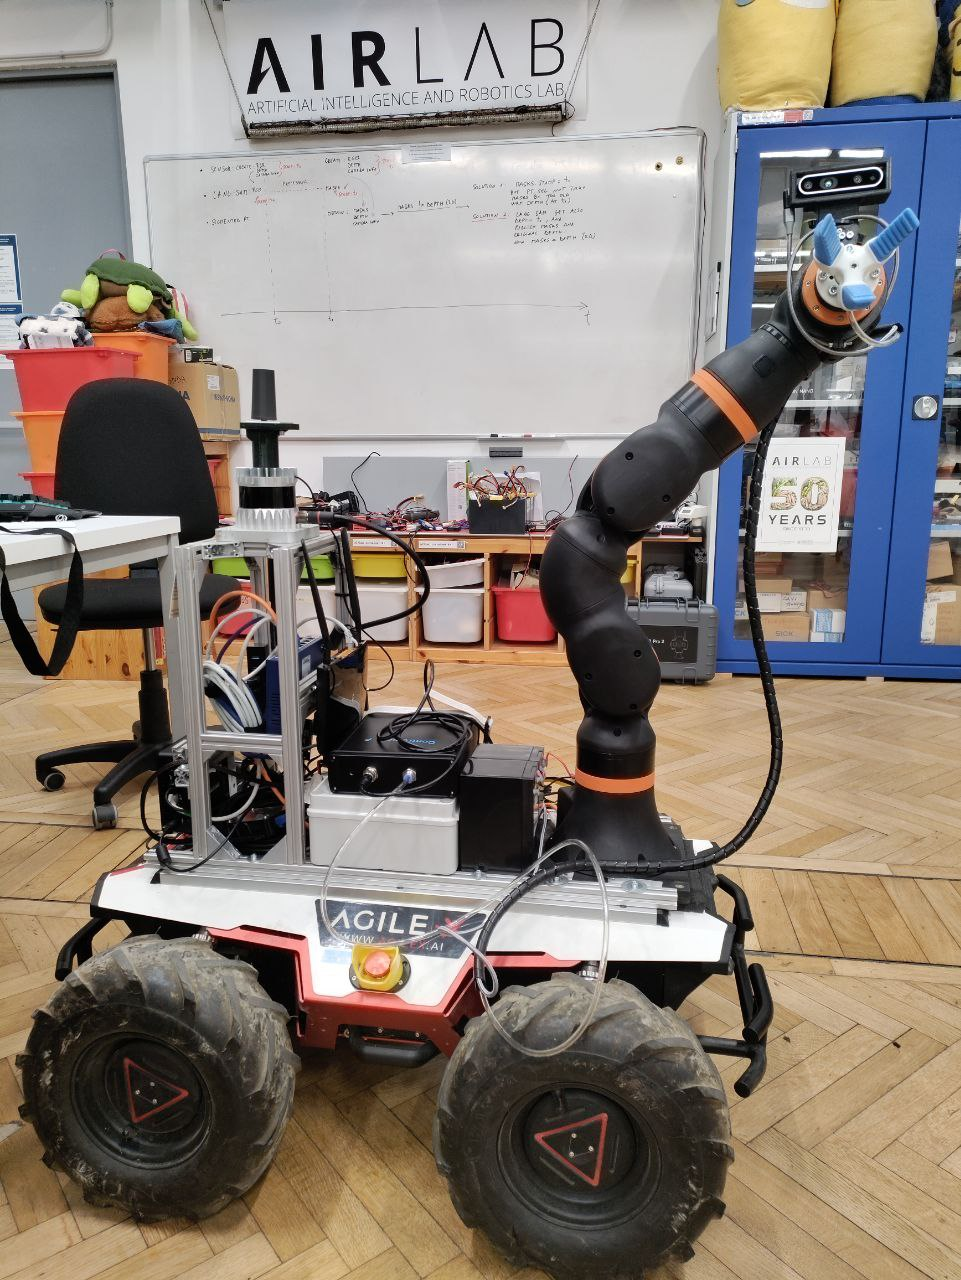
\includegraphics[width=0.8\textwidth]{c3_28.jpg}
    \captionsetup{width=1\linewidth}
    \caption{Lateral view of the robots}
    \label{fig:c3_img28}
\end{figure}